

% \vspace{-10pt}
\subsection{Limitations of Dictionary-Based Techniques} \label{sub:template}
\vspace{-5pt}


\begin{center}
\begin{figure}[h!]
\begin{subfigure}[b]{.33\textwidth}
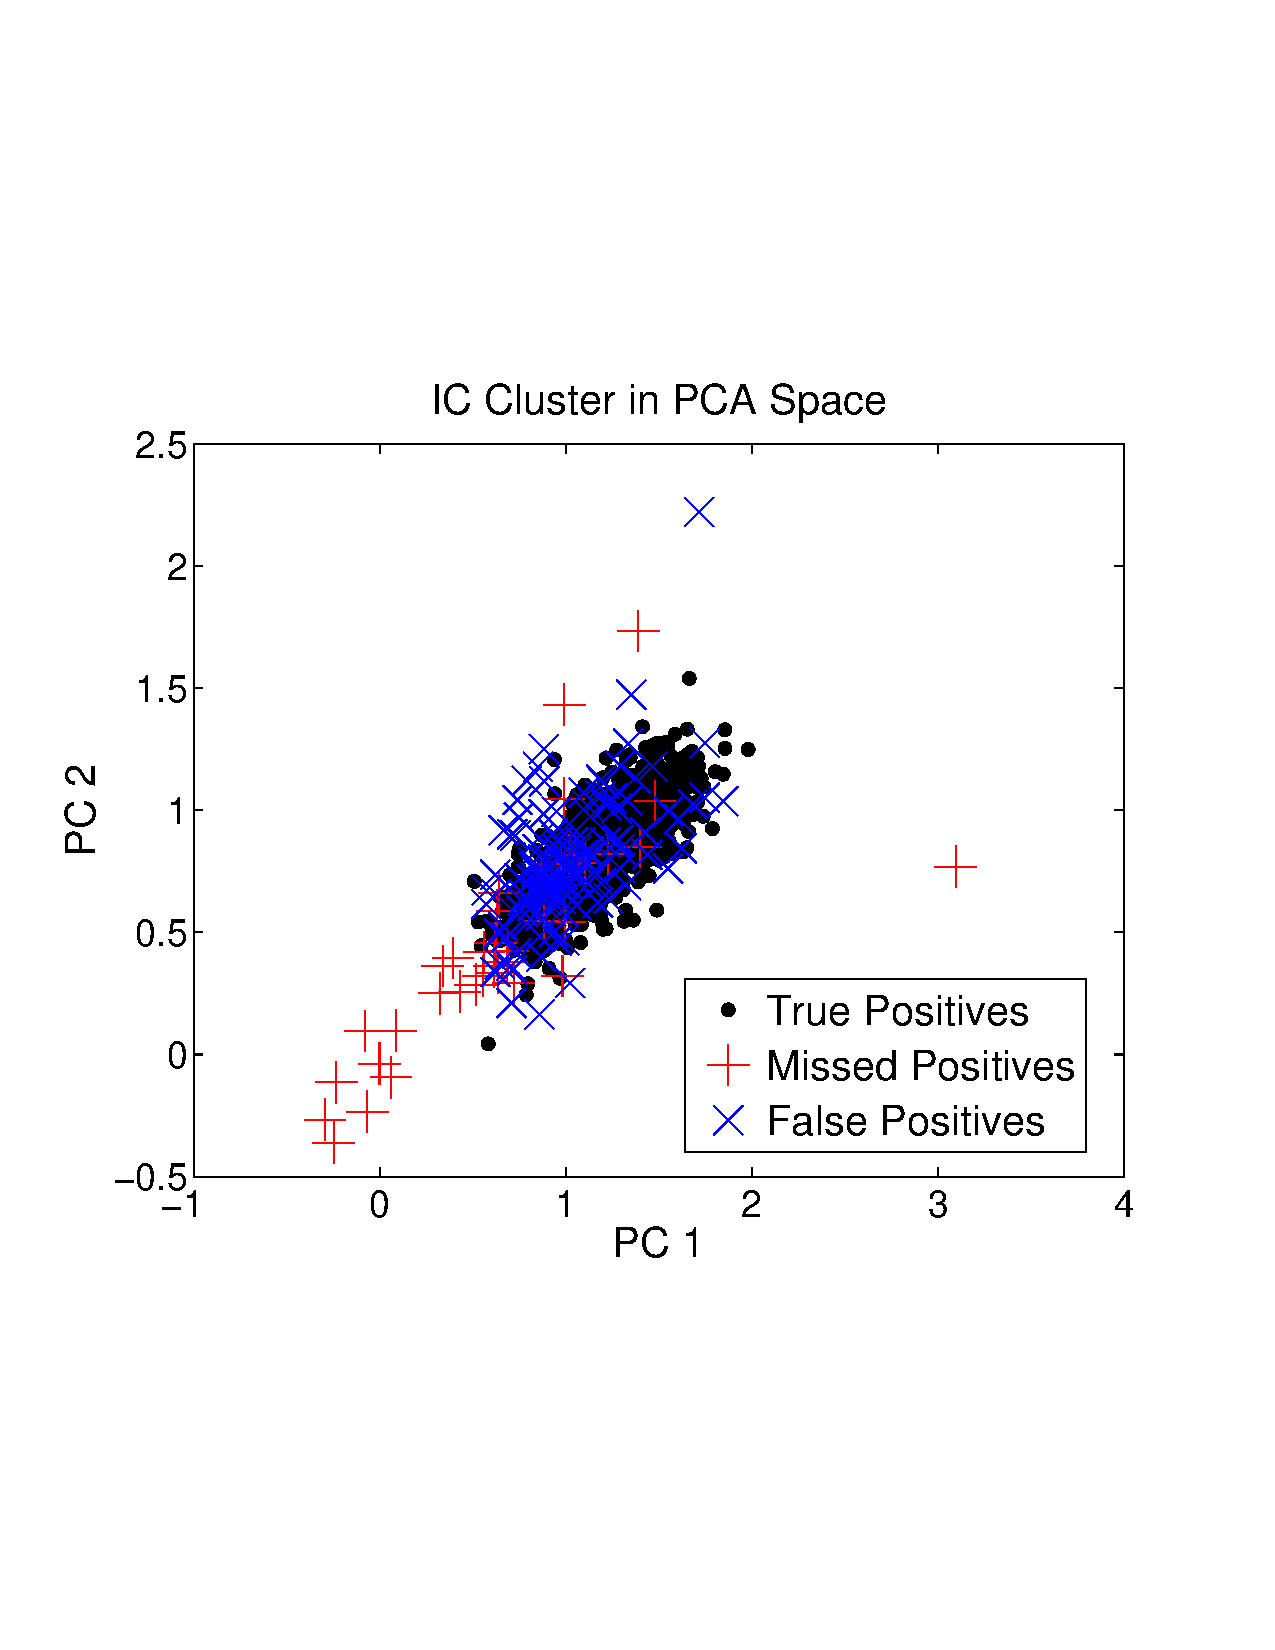
\includegraphics[width=\textwidth]{../figs/new/ICclusteroldpca.pdf}
\caption{}
\label{fig:ICold}
\end{subfigure}
\begin{subfigure}[b]{.33\textwidth}
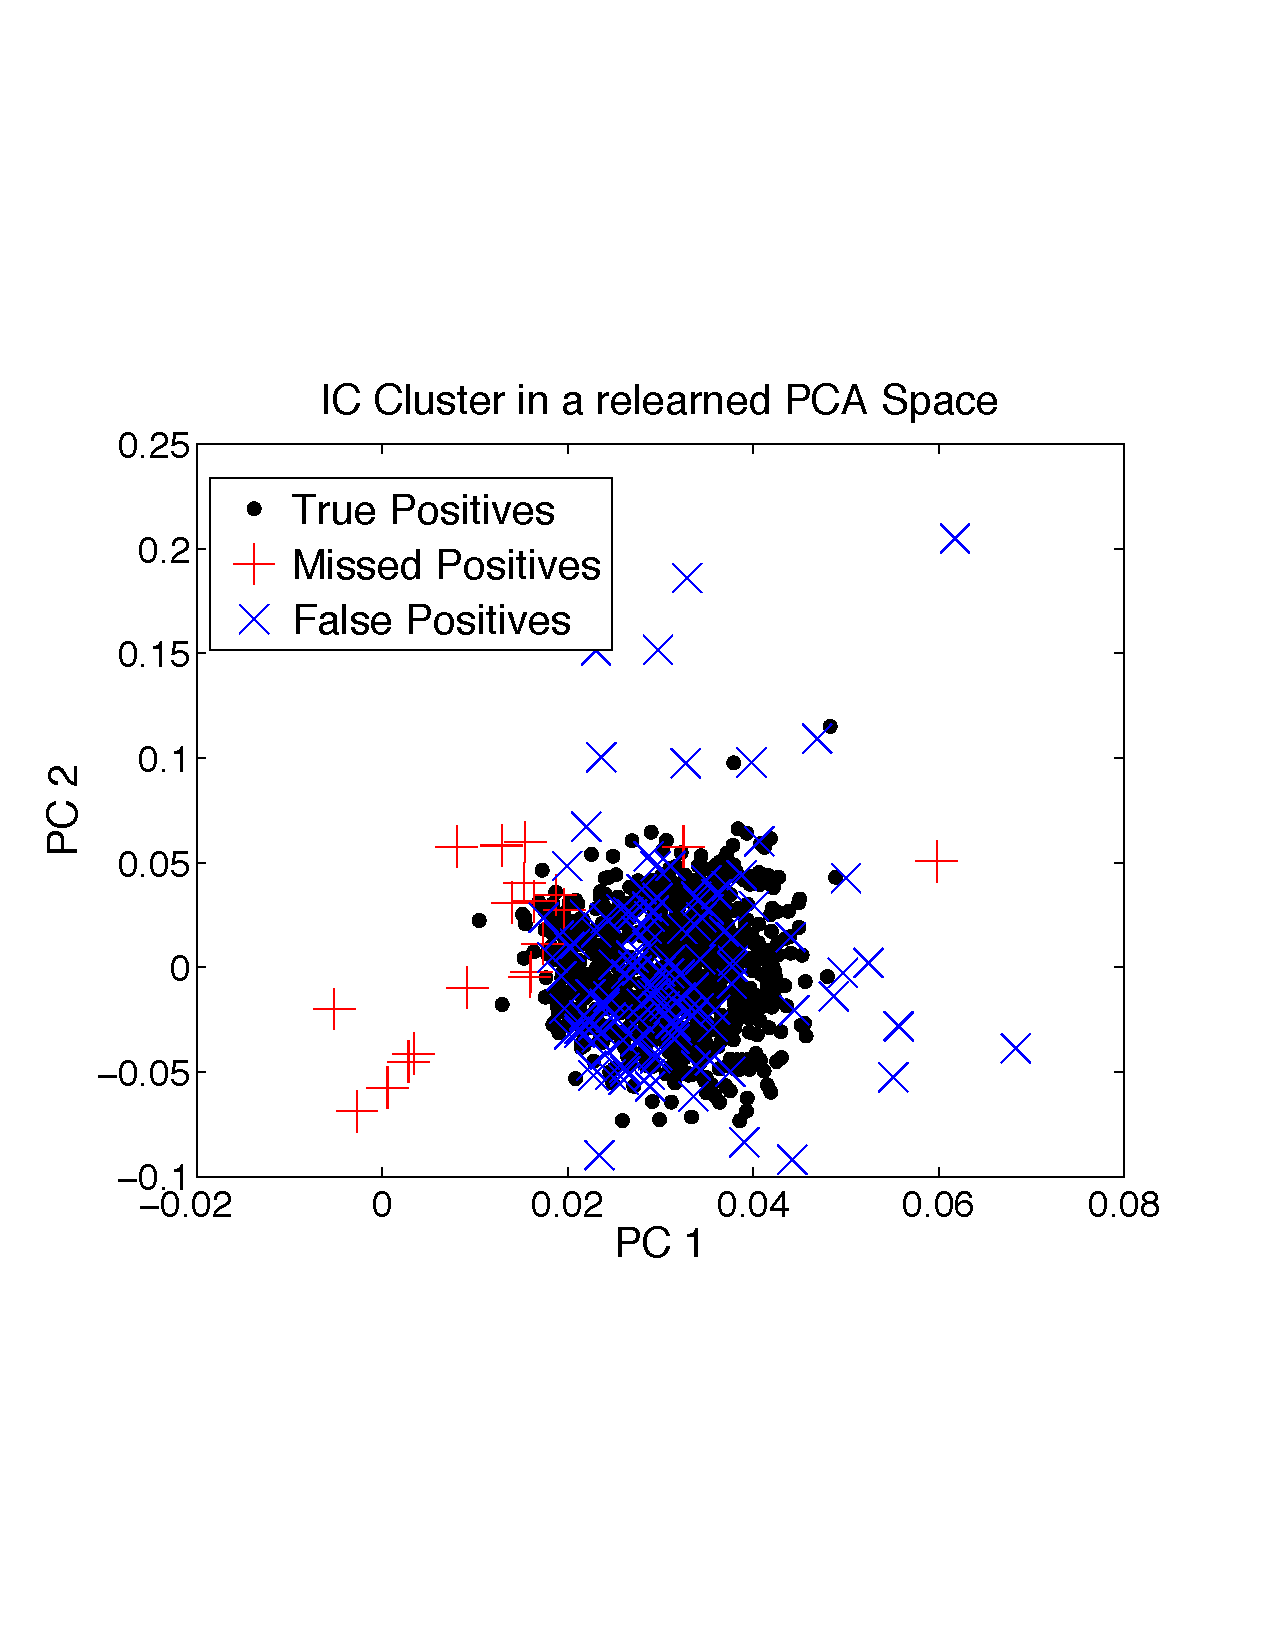
\includegraphics[width=\textwidth]{../figs/new/ICclusternewpca.pdf}
\caption{}
\label{fig:ICnew}
\end{subfigure}
\begin{subfigure}[b]{.33\textwidth}
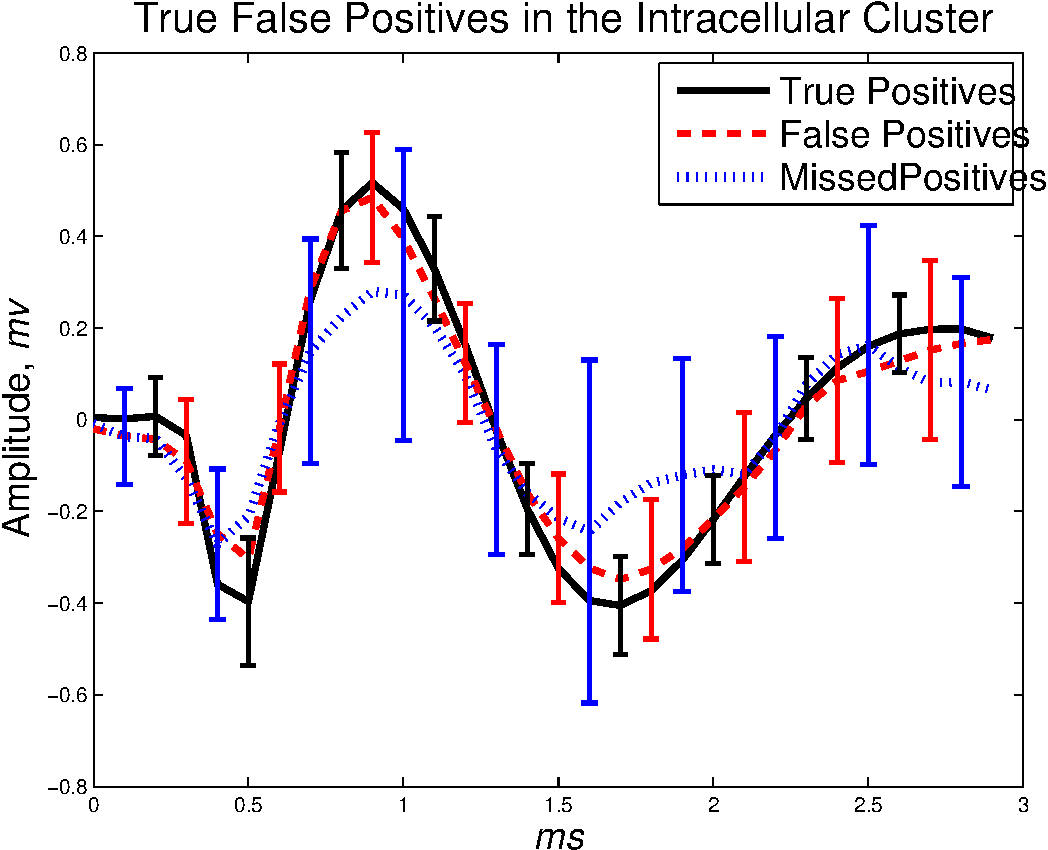
\includegraphics[width=\textwidth]{../figs/IntracellularTrueFalsePositivesv2}
\caption{}
\label{truewaveforms}
\end{subfigure}
\caption{Template matching.
(c) Errorbar plots of the true positives and the false positives in the IC cluster.  While the false positives have slightly more variability, the mean shape for the false positives and the true positives is nearly identical.  The true misses have a significantly lower amplitude as well as high variability. 
} \label{fig:IC-PCA}
\end{figure}
\end{center}




in discussion:

embarrassingly parallel per 4

ignore time steps that aren't useful

let $\lambda_i$ vary as a function of: (i) spike histories, (ii) stimulus, (iii) possibly baseline drift?


\clearpage
\section{comments}

{\color{red} perhaps add comments about time-evolution and the false positives we avoid by using multi-channel analysis}

\jovo{add grids to all panels of all figs by default, remove if it looks shitty.}

\jovo{@dec - for fig 1 keep colors/symbols the same in the two panel, if possible.  maybe use a scheme where color indicates algorithm and shape indicates \# of components.  also, be consistent about "IC" cluster vs. "Intracellular" Cluster. and normalize, renaming axes XY Rate instead of only XY. (b) title should be ``ROC Curve Comparisons''}  


